\chapter{Abbildungen}\label{apdx:A}

% Nummerierung auf A1, A2, etc. umstellen
\renewcommand{\thefigure}{A.\arabic{figure}}
\setcounter{figure}{0} % Zähler zurücksetzen

%\section{Abbildungen}\label{sec:apdx:Abbildungen}
\captionsetup[figure]{justification=raggedright, singlelinecheck=false, labelsep=colon}
\clearpage

\begin{figure}[H]
    \centering
    \begin{tikzpicture}
        % Bild um 90° drehen und auf Seitenhöhe skalieren
        \node[anchor=south west, inner sep=0] (image) at (0,0) 
            {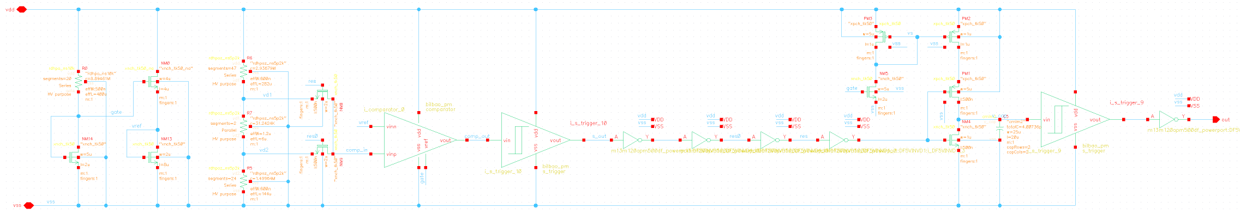
\includegraphics[keepaspectratio, scale=0.7, angle=-90]{figures/CD/Picture1.png}};

        % Berechnung der Mittelpunkte für die Beschriftung
        \pgfmathsetmacro{\ymidA}{(0 + 7)/2}
        \pgfmathsetmacro{\ymidB}{(7 + 13.5)/2}    % Mittelpunkt für "Schaltpunkte Komparator"
        \pgfmathsetmacro{\ymidC}{(13.5 + 18.5)/2} % Mittelpunkt für "Inverterkette"
        \pgfmathsetmacro{\ymidD}{(18.5 + 23)/2}   % Mittelpunkt für "Generierung Referenzstrom"

        \begin{scope}
            % Gestrichelte Linien
            \draw[dashed] (0,7) -- ++(10,0);
            \draw[dashed] (0,13.5) -- ++(10,0);
            \draw[dashed] (0,18.5) -- ++(10,0);

            % Mittelpunkte setzen (berechnete Werte werden nun genutzt)
            \node at (8, \ymidA) {\textbf{Verzögerungs- und Reset-Element}};
            \node at (8, \ymidB) {\textbf{Inverterkette}};
            \node at (8, \ymidC) {\textbf{Schaltpunkte Komparator}};
            \node at (8, \ymidD) {\textbf{Generierung Referenzstrom}};
        \end{scope}
    \end{tikzpicture}
    \caption{Schaltbild der kompletten PoR-Schaltung}
    \label{fig:PoR_complete}
\end{figure}


\begin{figure}[H]
    \centering
    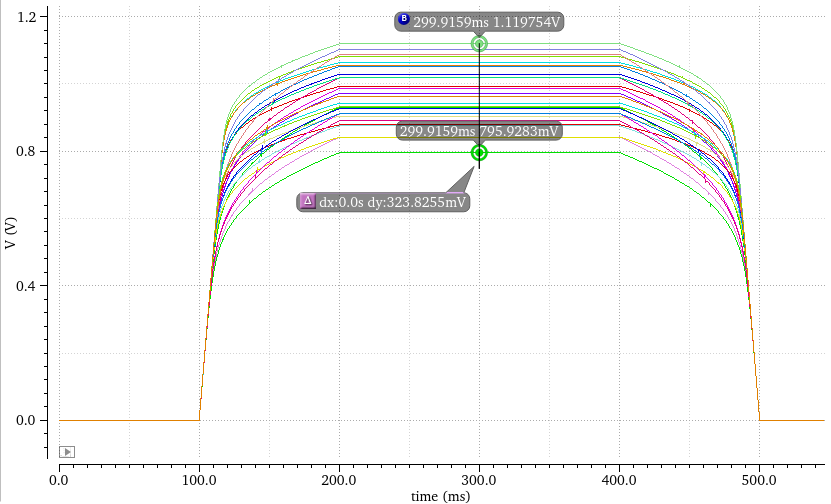
\includegraphics[width=\linewidth]{figures/CD/vref_old.png}
    \caption{Schwankung der Referenzspannung mit Widerstand}
    \label{fig:Vref_fluctuation_old}
    \addcontentsline{app}{figure}{\protect\numberline{\thefigure} Schwankung der Referenzspannung mit Widerstand}
\end{figure}

\begin{figure}[H]
    \centering
    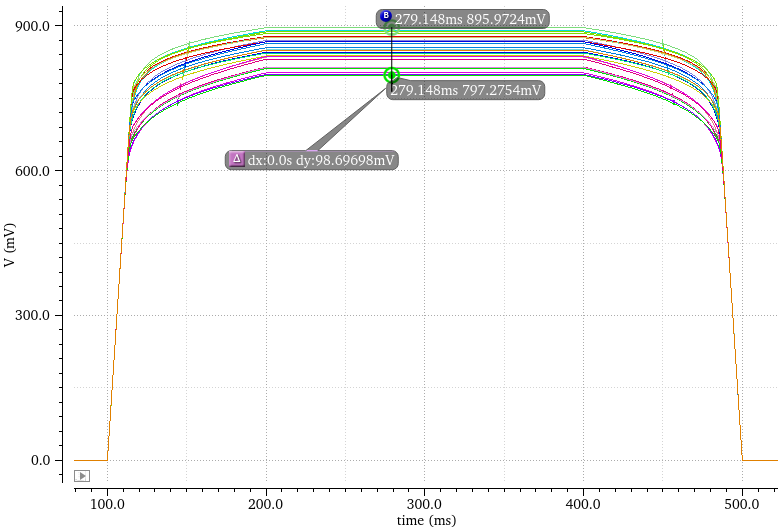
\includegraphics[width=\linewidth]{figures/CD/vref_test1.png}
    \caption{Schwankung der Referenzspannung mit Transistoren}
    \label{fig:Vref_Variation}
    \addcontentsline{app}{figure}{\protect\numberline{\thefigure} Schwankung der Referenzspannung mit Transistoren}
\end{figure}
